\section{Model Architecture}
\label{sec:model_arc}

\begin{figure}[t]
    \centering
    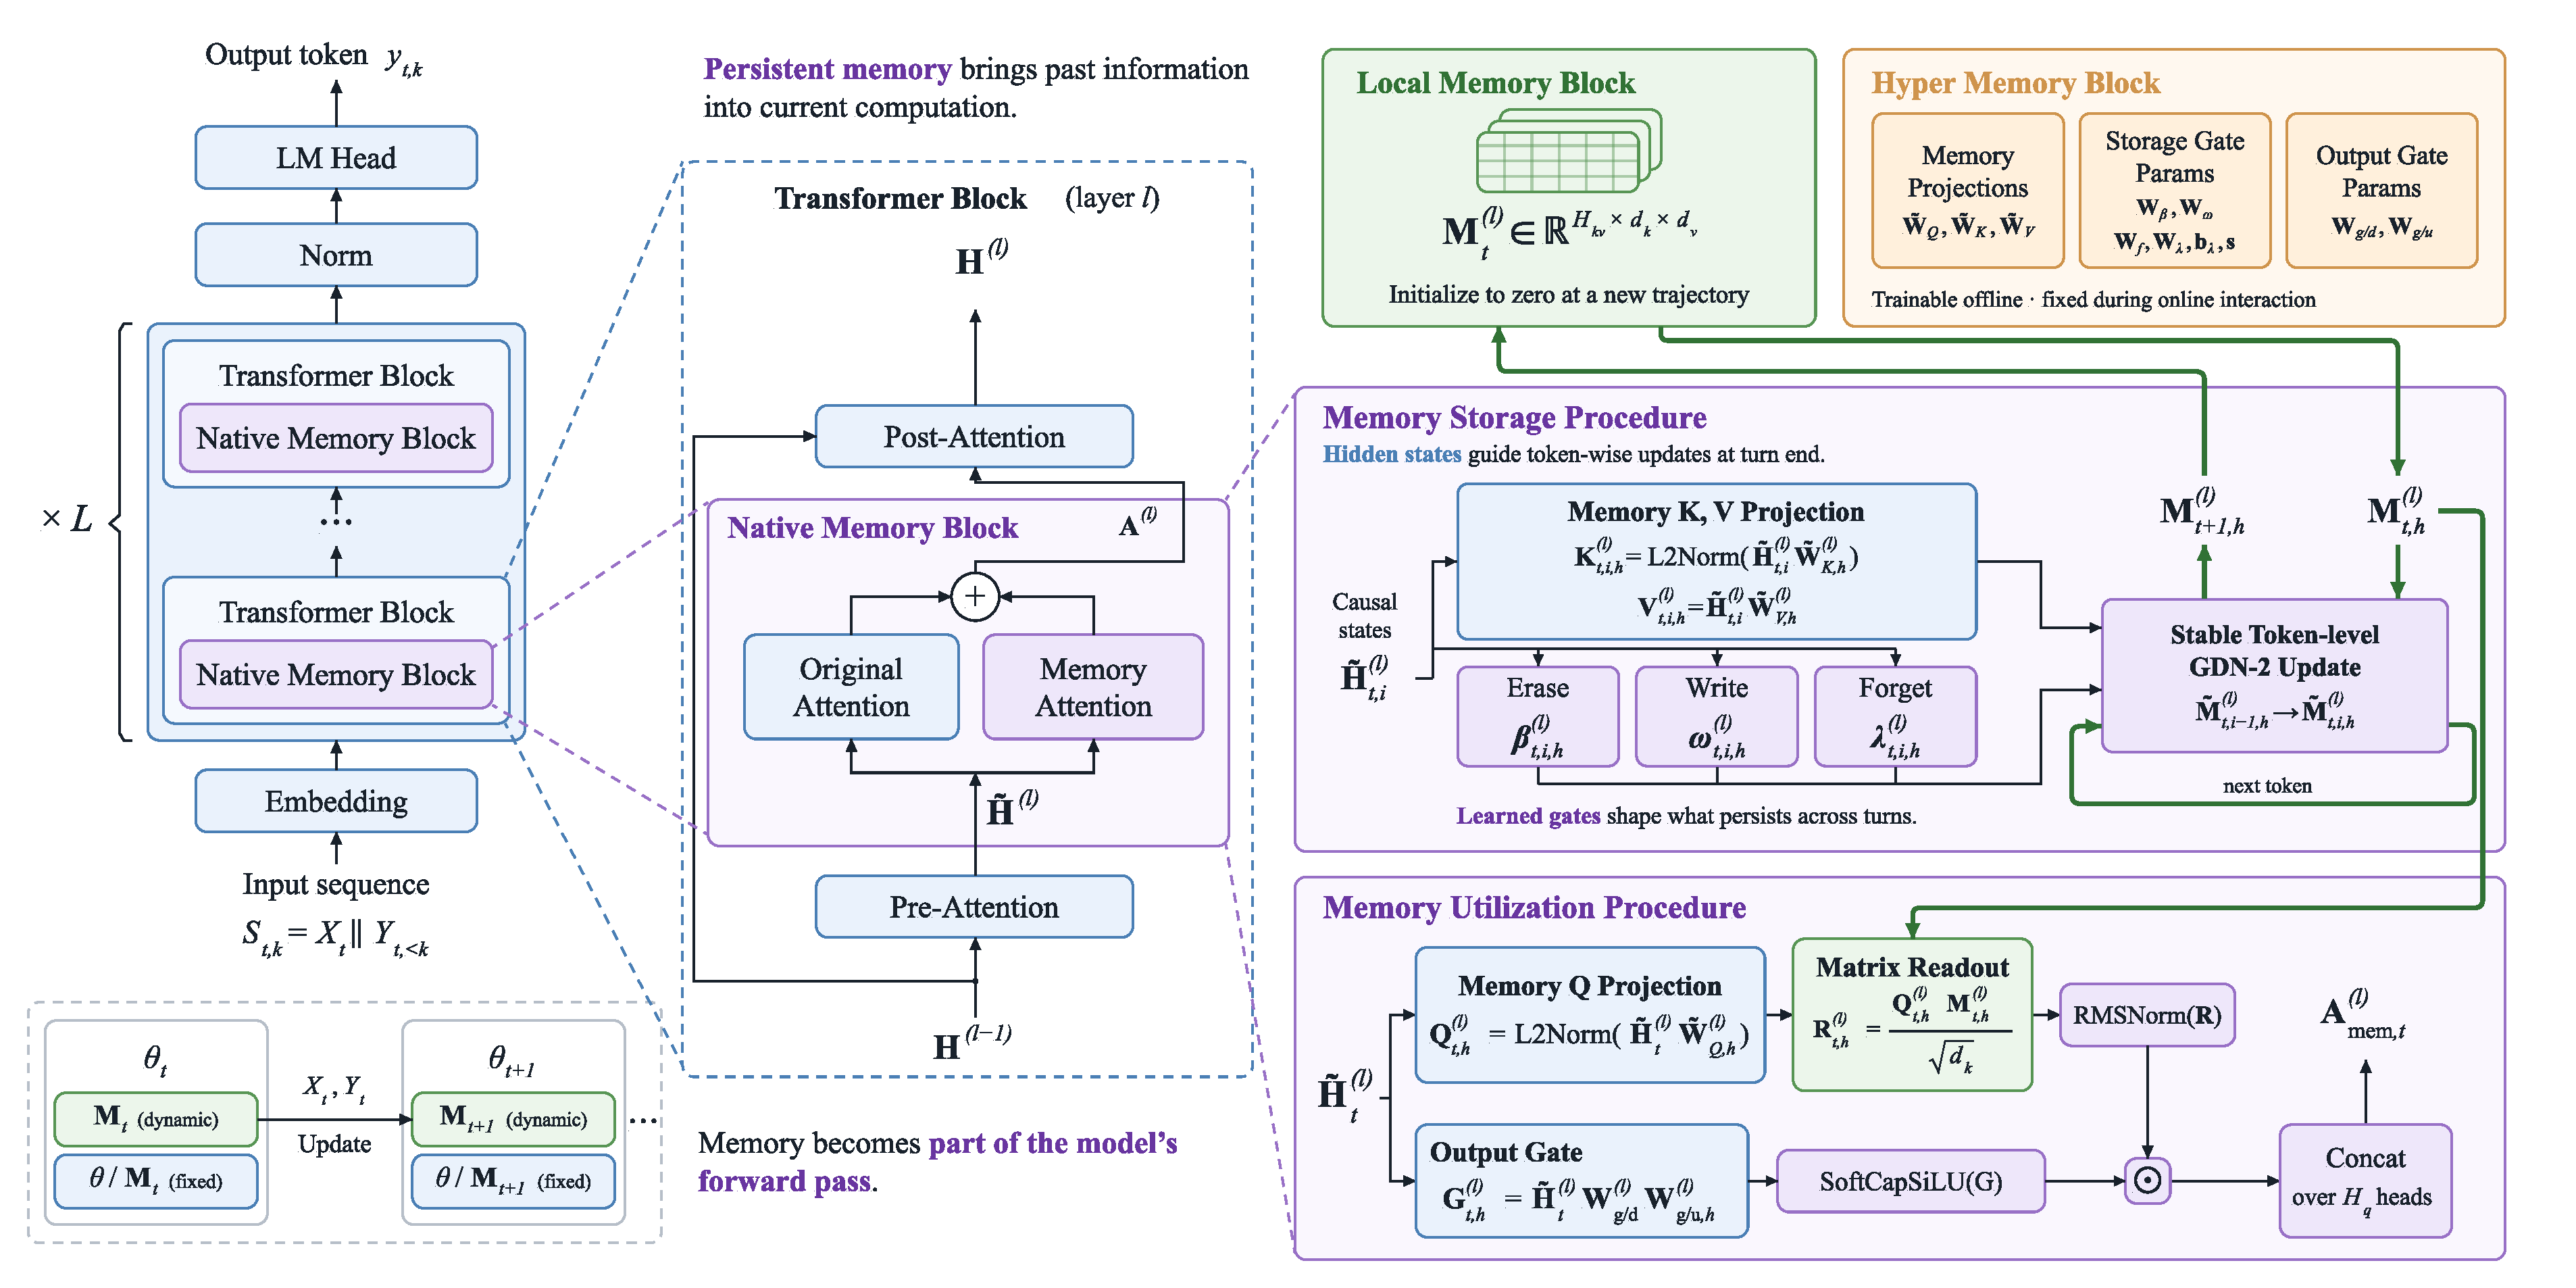
\includegraphics[width=\linewidth]{figures/memt-arc.pdf}
    \vspace{-0.6cm}
    \caption{Architecture of MemT-1.0. MemT-1.0 equips causal language models with native memory that evolves across interaction steps. Each selected Transformer block is augmented with a native memory block that performs parallel original and memory attention. The memory mechanism comprises dynamic local memory and trainable hyper memory, together with native memory storage and utilization procedures for updating and retrieving persistent information.}
    \label{fig:memt_arc}
    \vspace{-0.4cm}
\end{figure}

\subsection{Overview}
MemT-1.0 is formulated under a multi-step scenario with discrete steps $t \in \{1,2, \cdots, T\}$, as presented in Figure~\ref{fig:memt_arc}.
At step $t$, let $\theta_t$ denote the current model parameters.
Given the input $X_t$, the autoregressive generation process can be formulated as
\begin{equation*}
    y_{t,k} \sim P \left( \cdot | X_t,Y_{t,<k} ; \theta_t \right),
\end{equation*}
where $Y_{t,<k}$ denotes the tokens generated before $y_{t,k}$.
Meanwhile, the stateful model parameter is updated by
\begin{equation*}
    \theta_{t+1} \sim P\left( \cdot | X_t,Y_t ; \theta_t \right),
\end{equation*}
where $Y_{t}$ is all generated tokens at step $t$.
MemT-1.0 is built upon general causal language models.
We denote the input sequence as $S_{t,k} = X_t||Y_{t,<k} = \left(x_{t,1}, \cdots, y_{t,1}, \cdots , y_{t,k-1}\right)$ with length $L_{t,k}$.
First, the input is mapped to the initial hidden state $\mathbf{H}^{(0)}_{t,k} \in \mathbb{R}^{L_{t,k} \times d}$ through the embedding layer, where $d$ is the dimension of the hidden state.
Then, it is processed sequentially by $L$ stacked Transformer blocks~\cite{vaswani2017attention} as follows:
\begin{equation*}
    \mathbf{H}^{(l)}_{t,k} = \operatorname{TransformerBlock}\left( \mathbf{H}^{(l-1)}_{t,k} \right), \quad \text{for $l=1, 2, \cdots L$}.
\end{equation*}
After that, the last hidden state $\mathbf{H}^{(L)}_{t,k}$ is normalized and projected into the vocabulary space through the language modeling head $\mathbf{W}_{\text{LM}} \in \mathbb{R}^{d \times |\mathcal{V}|}$, and a softmax function is then applied to obtain the probability distribution by
\begin{equation*}
    P \left( \cdot | X_t,Y_{t,<k} ; \theta_t \right) = \Softmax \left( \Norm\left( \mathbf{h}^{(L)}_{t,k} \right) \mathbf{W}_{\text{LM}} \right),
\end{equation*}
where $|\mathcal{V}|$ is the vocabulary size and $\mathbf{h}^{(L)}_{t,k}$ is the last position of $\mathbf{H}^{(L)}_{t,k}$.

MemT-1.0 augments each selected standard Transformer block with a native memory block, which is responsible for maintaining the memory from previous information.
For the $l$-th Transformer block, we denote the computation of attention output as 
\begin{equation*}
    \mathbf{A}^{(l)}_{\text{ori},t,k} = \operatorname{Attention}\left(\tilde{\mathbf{H}}^{(l)}_{t,k} \right), \quad \tilde{\mathbf{H}}^{(l)}_{t,k} = \operatorname{Pre-Attention}\left({\mathbf{H}}^{(l-1)}_{t,k} \right),
\end{equation*}
where $\operatorname{Attention}\left( \cdot \right)$ represents the backbone attention and $\tilde{\mathbf{H}}^{(l)}$ indicates the hidden state after pre-attention operations, such as pre-normalization.
MemT-1.0 introduces a parallel memory attention mechanism to utilize the parametric memory accumulated from previous steps for targeted layers, by
\begin{equation*}
    \mathbf{A}^{(l)}_{t,k} = \mathbf{A}^{(l)}_{\text{ori},t,k} + \mathbf{A}^{(l)}_{\text{mem},t,k}, \quad \mathbf{A}^{(l)}_{\text{mem},t,k} = \operatorname{MemoryAttention}\left( \tilde{\mathbf{H}}^{(l)}_{t,k}; \cdot \right),
\end{equation*}
where $\mathbf{A}^{(l)}_{\text{mem},t,k}$ indicates the output of memory attention.
After that, the combined attention output $\mathbf{A}^{(l)}_{t,k}$ is used in the subsequent computation as
\begin{equation*}
    \mathbf{H}^{(l)}_{t,k} = \operatorname{Post-Attention}\left( \mathbf{A}^{(l)}_{t,k}, {\mathbf{H}}^{(l-1)}_{t,k} \right).
\end{equation*}
For different backbones, we preserve the original $\operatorname{Pre-Attention}\left( \cdot \right)$, $\operatorname{Attention}\left( \cdot \right)$, and $\operatorname{Post-Attention}\left( \cdot \right)$ unchanged to retain the backbone capabilities, and introduce memory through $\operatorname{MemoryAttention}\left( \cdot \right)$ for different backbones.
Specifically, we use Qwen3.6-35B-A3B~\cite{qwen36_35b_a3b}, as released, as the backbone of MemT-1.0-Nano and a further post-trained DeepSeek-V4-Flash~\cite{deepseekai2026deepseekv4} (Section~\ref{sec:backbone_prep}) as the backbone of MemT-1.0-Flash.

\subsection{Native Memory Block}

\subsubsection{Native Memory State}

Following our previous work Metis~\cite{zhang2026metis}, a native memory block in MemT-1.0 comprises a local memory block and a hyper memory block.
The former stores online information, while the latter is trained to equip general foundation models with memory capabilities in a data-driven manner.

\textbf{Local Memory Block.}
In MemT-1.0, the dynamic memory state at the $t$-th step and $l$-th layer can be represented as $\mathbf{M}_t^{(l)} \in \mathbb{R}^{H_{kv} \times d_k \times d_v}$, where $d_k, d_v$ represent the dimensions of memory keys and values, and $H_{kv}$ denotes the number of memory channels.
Compared with Metis, we remove the query-key normalization vector and extend the memory state to multiple channels. 
We initialize $\mathbf{M}_t^{(l)} = \mathbf{0}$ at the start of new trajectories.

\textbf{Hyper Memory Block.}
In the hyper memory block, the multi-channel projections of memory query, key, and value are denoted as $\tilde{\mathbf{W}}_Q^{(l)} \in \mathbb{R}^{H_{q} \times d \times d_k}$, $\tilde{\mathbf{W}}_K^{(l)} \in \mathbb{R}^{H_{kv} \times d \times d_k}$ and $\tilde{\mathbf{W}}_V^{(l)} \in \mathbb{R}^{H_{kv} \times d \times d_v}$ for each layer $l$.
Beyond these core memory projections, this block includes all other trainable parameters for memory processing.
First, the gating projections include the erase gate $\mathbf{W}_{\beta}^{(l)} \in \mathbb{R}^{d \times H_{kv} \times d_k}$ and the write gate $\mathbf{W}_{\omega}^{(l)} \in \mathbb{R}^{d \times H_{kv} \times d_v}$, along with the forget gate components consisting of $\mathbf{W}_{f}^{(l)} \in \mathbb{R}^{d \times d_{\text{gate}}}$, $\mathbf{W}_{\lambda}^{(l)} \in \mathbb{R}^{d_{\text{gate}} \times H_{kv} \times d_k}$, $\mathbf{b}_{\lambda}^{(l)} \in \mathbb{R}^{H_{kv} \times d_k}$, and a learnable vector $\mathbf{s}^{(l)} \in \mathbb{R}^{H_{kv}}$.
Finally, the memory output gating is parameterized by a shared down-projection $\mathbf{W}_{g/d}^{(l)} \in \mathbb{R}^{d \times d_{g/d}}$ and a multi-channel up-projection $\mathbf{W}_{g/u}^{(l)} \in \mathbb{R}^{H_q \times d_{g/d} \times d_v}$.
Generally, we have $H_q = H_{kv}$ to align query channel and key-value channels. 
These trainable parameters are denoted as $\phi$, which can be optimized during the training phase and remain fixed during online interaction.

In summary, the model parameters $\theta_t$ at step $t$ include the backbone parameters $\theta_b$, the static but trainable parameters $\phi$, and the dynamic memory states $\{\mathbf{M}_t^{(l)}\}_{l=1}^{L}$.
During online inference, these dynamic memory states are responsible for storing online information and evolve over interactions.

\subsubsection{Native Memory Procedures}
MemT-1.0 consists of two parallel native procedures, including memory storage and memory utilization.
The memory storage procedure updates the dynamic memory states to preserve information from the current interaction, while the memory utilization procedure retrieves information from previously accumulated memory states to support autoregressive generation.

\textbf{Native Memory Storage Procedure.}
MemT-1.0 replaces the token selection with a stable token-level update mechanism based on GDN-2~\cite{hatamizadeh2026gated} to update the dynamic memory state in each turn.
As the memory storage procedure is triggered at the turn level, we denote the hidden states as $\mathbf{H}^{(l)}_t$ of $S_{t} = X_t||Y_t$.
For the pre-attention input $\tilde{\mathbf{H}}^{(l)}_t$, we compute the memory key and value of the $h$-th channel by
\begin{equation*}
    \mathbf{K}_{t,h}^{(l)} = \operatorname{L2Norm}\left(\tilde{\mathbf{H}}^{(l)}_{t} \tilde{\mathbf{W}}_{K,h}^{(l)}\right), \quad \mathbf{V}_{t,h}^{(l)} = \tilde{\mathbf{H}}^{(l)}_{t} \tilde{\mathbf{W}}_{V,h}^{(l)},
\end{equation*}
where $\tilde{\mathbf{W}}_{K,h}^{(l)}$ and
$\tilde{\mathbf{W}}_{V,h}^{(l)}$ are the key and value projection matrices for the $h$-th memory channel.
Then, the erase gate and write gate can be obtained by
\begin{equation*}
    \bm{\beta}_{t}^{(l)} = \sigma\left( \tilde{\mathbf{H}}^{(l)}_{t} \mathbf{W}_{\beta}^{(l)} \right),
    \quad \bm{\omega}_{t}^{(l)} = \sigma\left( \tilde{\mathbf{H}}^{(l)}_{t} \mathbf{W}_{\omega}^{(l)} \right),
\end{equation*}
where $\mathbf{W}_{\beta}^{(l)}, \mathbf{W}_{\omega}^{(l)}$ are gating projection matrices.
In addition, the forget gate is calculated by
\begin{equation*}
    \bm{\lambda}_{t,h}^{(l)} = - \exp \left(\mathbf{s}^{(l)}_{h} \right) \odot \operatorname{Softplus}\left( \mathbf{F}_{t}^{(l)} \mathbf{W}_{\lambda,h}^{(l)} +\mathbf{b}_{\lambda,h}^{(l)} \right),
    \quad \mathbf{F}_{t}^{(l)} = \tilde{\mathbf{H}}^{(l)}_{t} \mathbf{W}_{f}^{(l)} ,
\end{equation*}
where $\mathbf{W}_{f}^{(l)}, \mathbf{W}_{\lambda}^{(l)}, \mathbf{b}_{\lambda}^{(l)}, \mathbf{s}_h^{(l)}$ are forget-gate parameters.
To prevent the divergence of memory states during updates, we introduce a stable mechanism for the token-level update, where it first calculates
\begin{equation*}
    \mathbf{U}_{t,i}^{(l)} = \sqrt{\bm{\beta}_{t,i}^{(l)}}
\odot
\mathbf{K}_{t,i}^{(l)}.
\end{equation*}
Then, the memory state can be updated by
\begin{equation*}
    \tilde{\mathbf{M}}_{t, i, h}^{(l)} = \left[
\mathbf{I}
-
\mathbf{U}_{t,i,h}^{(l)\top}
\mathbf{U}_{t,i,h}^{(l)}
\right]
\cdot
\mathbf{D}_{t,i,h}^{(l)}
\tilde{\mathbf{M}}_{t,i-1,h}^{(l)}
+
\mathbf{U}_{t,i,h}^{(l)\top}
\left(
\bm{\omega}_{t,i,h}^{(l)}
\odot
\mathbf{V}_{t,i,h}^{(l)}
\right),
\end{equation*}
where the initialization is given by $\tilde{\mathbf{M}}_{t, 0, h}^{(l)} = \mathbf{M}_{t,  h}^{(l)}$, and the state transition is defined as $\mathbf{M}_{t+1,  h}^{(l)} = \tilde{\mathbf{M}}_{t, L_t, h}^{(l)}$, with
\begin{equation*}
    \mathbf{D}_{t,i,h}^{(l)} = \operatorname{Diag}
\left[
\exp
\left(
\bm{\lambda}_{t,i,h}^{(l)}
\right)
\right].
\end{equation*}
The detailed analysis of our stable mechanism on GDN-2 is presented in Appendix~\ref{appendix:stable_gdn2}.

\textbf{Native Memory Utilization Procedure.}
In MemT-1.0, we remove the key-value normalization from Metis.
Because the memory utilization operates at the token level in parallel, we omit the decoding index $k$ for simplicity.
For the step $t$, we read out information from the current memory state $\mathbf{M}_{t,h}^{(l)}$ by
\begin{equation*}
    \mathbf{R}_{t,h}^{(l)} = \frac{\mathbf{Q}_{t,h}^{(l)} \mathbf{M}_{t,h}^{(l)}}{\sqrt{d_k}}, 
    \quad \mathbf{Q}_{t,h}^{(l)} = \operatorname{L2Norm}\left(\tilde{\mathbf{H}}^{(l)}_{t} \tilde{\mathbf{W}}_{Q,h}^{(l)}\right),
\end{equation*}
where $\tilde{\mathbf{W}}_{Q,h}^{(l)}$ is the memory query projection matrix.
After that, we calculate the memory output gate by 
\begin{equation*}
    \mathbf{G}_{t,h}^{(l)} = \tilde{\mathbf{H}}^{(l)}_{t} \mathbf{W}_{g/d}^{(l)} \mathbf{W}_{g/u,h}^{(l)},
\end{equation*}
where $\mathbf{W}_{g/d}^{(l)},\mathbf{W}_{g/u,h}^{(l)}$ are parameters of the readout gate.
Finally, the memory attention is calculated by
\begin{equation*}
    \begin{aligned}
        \mathbf{A}_{\text{mem},t}^{(l)} & = \operatorname{MemoryAttention}\left( \tilde{\mathbf{H}}^{(l)}_{t,k}; \mathbf{M}_{t}^{(l)} \right) \\
        & = \operatorname{Concat}_{h=1}^{H_{q}}\left[ \operatorname{RMSNorm}\left( \mathbf{R}_{t,h}^{(l)} \right) \odot \operatorname{SoftCapSiLU}\left( \mathbf{G}_{t,h}^{(l)}\right) \right],
    \end{aligned}
\end{equation*}
where
\begin{equation*}
    \operatorname{SoftCapSiLU}(x)
    =
    \tau \tanh\left(
        \frac{\operatorname{SiLU}(x)}{\tau}
    \right),
    \qquad
    \operatorname{SiLU}(x) = x\,\sigma(x),
\end{equation*}
and $\tau > 0$ controls the soft-cap threshold, with $\tau = 2$ by default.
Target layers, projection strategies, and other settings vary slightly to accommodate different backbones, and more details can be found in Appendix~\ref{appendix:backbone_adaptation}.

\subsection{Scaling Native Memory Capacity}

\begin{figure}[t]
    \centering
    \vspace{-0.4cm}
    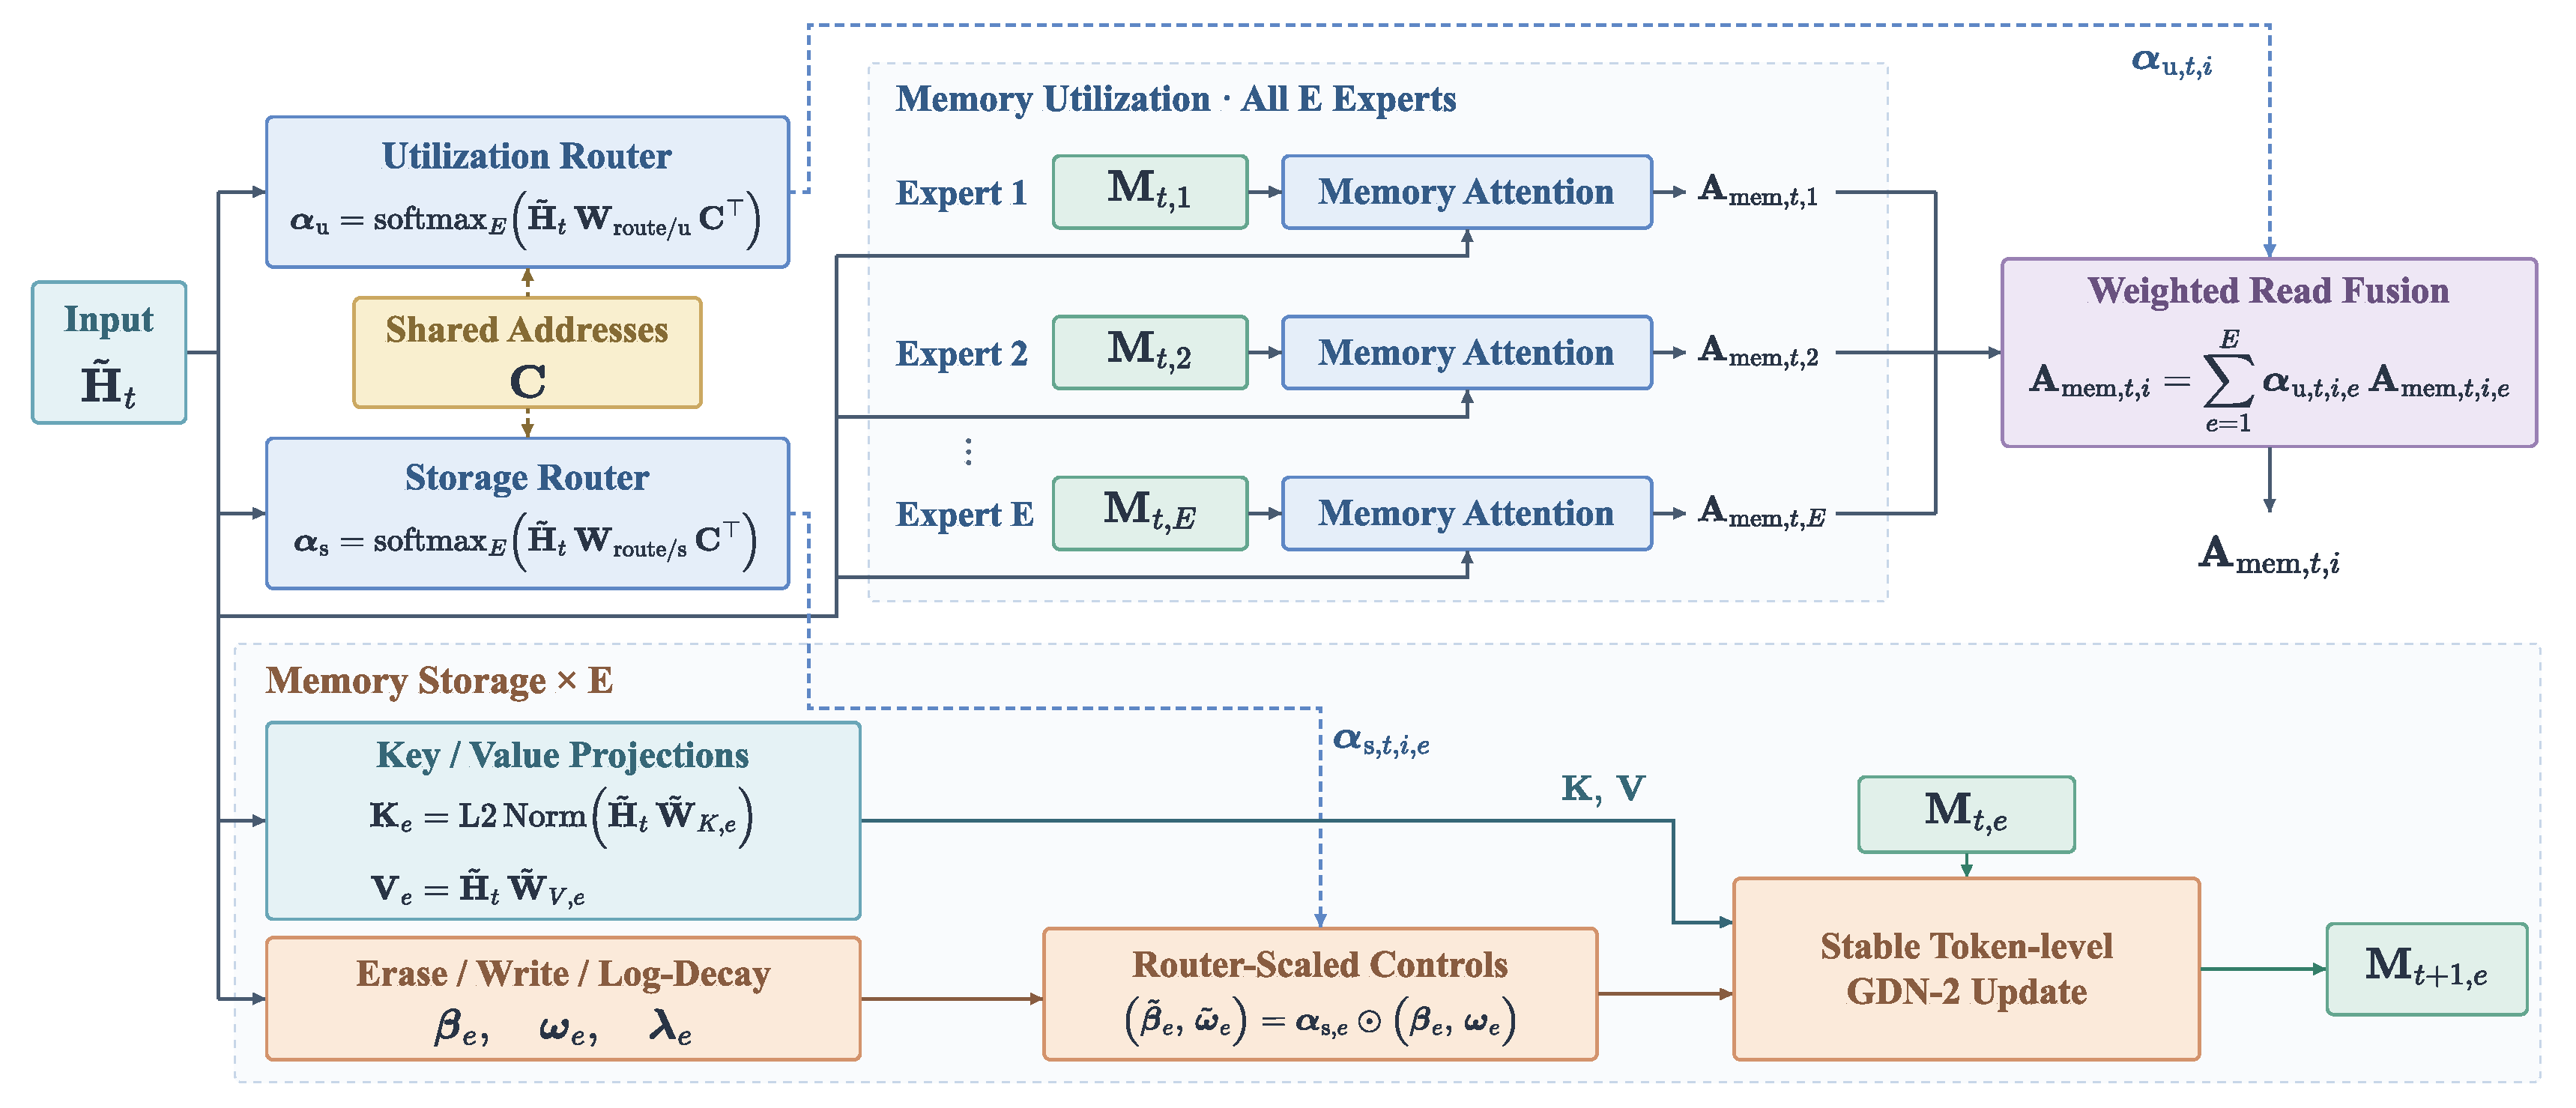
\includegraphics[width=\linewidth]{figures/memt-mos.pdf}
    \caption{Scaling native memory capacity. MoS expands each native memory block into multiple memory experts and employs separate dense storage and utilization routing over shared expert addresses.}
    \vspace{-0.4cm}
    \label{fig:mos_dse}
\end{figure}

To jointly scale the online memory capacity and the trainable memory parameters, we introduce Mixture-of-Storage (MoS), as presented in Figure~\ref{fig:mos_dse}, which expands a native memory block into $E$ parallel memory experts.
Unlike conventional sparse Mixture-of-Experts (MoE)~\cite{shazeer2017outrageouslylargeneuralnetworks}, MoS adopts dense routing over all memory experts, so every expert participates in the memory computation and the routing probabilities determine how information is read from and written into different memory experts.

\textbf{Memory Expert Expansion.}
For the $l$-th MoS layer, we extend the local memory state with an additional expert dimension as
\begin{equation*}
    \bm{\mathcal{M}}_{t,\mathrm{MoS}}^{(l)}
    =
    \left\{
    \mathbf{M}_{t,e}^{(l)}
    \right\}_{e=1}^{E}
    \in
    \mathbb{R}^{E \times H_{kv} \times d_k \times d_v},
\end{equation*}
where $\mathbf{M}_{t,e}^{(l)} \in \mathbb{R}^{H_{kv} \times d_k \times d_v}$ is the dynamic memory state of the $e$-th expert, and each expert has independent hyper memory parameters.
All experts and both routers receive the same pre-attention hidden states $\tilde{\mathbf{H}}_t^{(l)}$.

\textbf{Shared-Address Routing.}
MoS introduces two dense routers to control memory utilization and memory storage separately, which share a trainable expert address matrix
\begin{equation*}
    \mathbf{C}^{(l)}
    =
    \left[
    \mathbf{c}_{1}^{(l)},
    \mathbf{c}_{2}^{(l)},
    \cdots,
    \mathbf{c}_{E}^{(l)}
    \right]^\top
    \in
    \mathbb{R}^{E \times d_{\mathrm{addr}}},
\end{equation*}
where $d_{\mathrm{addr}}$ is the dimension of the address representation.
Then, we use router projections $\mathbf{W}_{\text{route/u}}^{(l)},\mathbf{W}_{\text{route/s}}^{(l)}
\in\mathbb{R}^{d\times d_{\mathrm{addr}}}$ for memory utilization and storage separately.
After that, routing probabilities of memory utilization are calculated by
\begin{equation*}
    \bm{\alpha}_{\text{u},t}^{(l)}
    =
    \Softmax
    \left(
    \tilde{\mathbf{H}}_{t}^{(l)}
    \mathbf{W}_{\text{route/u}}^{(l)}
    \mathbf{C}^{(l)\top}
    \right)
    \in\mathbb{R}^{L_t\times E}.
\end{equation*}
Similarly, routing probabilities of memory storage are obtained by
\begin{equation*}
    \bm{\alpha}_{\text{s},t}^{(l)}
    =
    \Softmax
    \left(
    \tilde{\mathbf{H}}_{t}^{(l)}
    \mathbf{W}_{\text{route/s}}^{(l)}
    \mathbf{C}^{(l)\top}
    \right)
    \in\mathbb{R}^{L_t\times E}.
\end{equation*}
Both softmax operations are applied along the expert dimension.
Therefore, the utilization and storage routers share the same semantic expert addresses but learn different projections.

\textbf{Mixture-of-Storage Fusion.}
For memory utilization, each expert independently follows the native memory utilization procedure described above.
We denote the memory-attention output of the $e$-th memory expert by
\begin{equation*}
    \mathbf{A}_{\mathrm{mem},t,e}^{(l)}
    =
    \operatorname{MemoryAttention}_{e}
    \left(
    \tilde{\mathbf{H}}_{t}^{(l)};
    \mathbf{M}_{t,e}^{(l)}
    \right).
\end{equation*}
The final memory attention at the $i$-th token in sequence $S_t$ is obtained by
\begin{equation*}
    \mathbf{A}_{\mathrm{mem},t,i}^{(l)}
    =
    \sum_{e=1}^{E}
    \bm{\alpha}_{\text{u},t,i,e}^{(l)}
    \mathbf{A}_{\mathrm{mem},t,i,e}^{(l)}.
\end{equation*}
For memory storage, each expert independently produces its memory key, value, erase gate, write gate, and log-decay using its expert-specific parameters.
For the $e$-th expert, the erase gate, write gate, and log-decay are calculated by
\begin{equation*}
    \tilde{\bm{\beta}}_{t,e}^{(l)}
    =
    \bm{\alpha}_{\text{s},t,e}^{(l)}
    \odot
    \bm{\beta}_{t,e}^{(l)},
    \qquad
    \tilde{\bm{\omega}}_{t,e}^{(l)}
    =
    \bm{\alpha}_{\text{s},t,e}^{(l)}
    \odot
    \bm{\omega}_{t,e}^{(l)},
    \qquad
    \tilde{\bm{\lambda}}_{t,e}^{(l)}
    =
    \bm{\lambda}_{t,e}^{(l)}.
\end{equation*}
After that, we calculate
\begin{equation*}
    \mathbf{U}_{t,e}^{(l)} = \sqrt{\tilde{\bm{\beta}}_{t,e}^{(l)}}
\odot
\mathbf{K}_{t,e}^{(l)}.
\end{equation*}
Finally, the memory state can be updated by
\begin{equation*}
    \tilde{\mathbf{M}}_{t,i,e,h}^{(l)} = \left[
\mathbf{I}
-
\mathbf{U}_{t,i,e,h}^{(l)\top}
\mathbf{U}_{t,i,e,h}^{(l)}
\right]
\cdot
\tilde{\mathbf{D}}_{t,i,e,h}^{(l)}
\tilde{\mathbf{M}}_{t,i-1,e,h}^{(l)}
+
\mathbf{U}_{t,i,e,h}^{(l)\top}
\left(
\tilde{\bm{\omega}}_{t,i,e,h}^{(l)}
\odot
\mathbf{V}_{t,i,e,h}^{(l)}
\right),
\end{equation*}
where we have the initialization $\tilde{\mathbf{M}}_{t, 0, e, h}^{(l)} = \mathbf{M}_{t, e, h}^{(l)}$, and transformation $\mathbf{M}_{t+1, e, h}^{(l)} = \tilde{\mathbf{M}}_{t, L_t, e, h}^{(l)}$, with
\begin{equation*}
    \tilde{\mathbf{D}}_{t,i,e,h}^{(l)} = \operatorname{Diag}
\left[
\exp
\left(
\tilde{\bm{\lambda}}_{t,i,e,h}^{(l)}
\right)
\right].
\end{equation*}

